\centerline{\bf \Huge Введение в переменную I}

\problem{1}
Доктор Айболит раздал четырём заболевшим зверям 2006 чудодейственных таблеток. Кощей получил на одну таблетку больше, чем кикимора, Баба Яга на одну больше, чем Кощей, а Змей Горыныч - на одну больше, чем Баба Яга. Сколько таблеток придётся съесть Змею Горынычу?

\textbf{Ответ:} Змей Горыныч получил 503 таблетки.

\textbf{Решение:}
Пусть Змей Горыныч получил а таблеток, тогда Баба Яга получила $(а-1)$ паблетку, значит Кощей получил $(a-1)-1$ таблеток или $(a-2)$ таблетки, наконец, сикимора получила $(a-3)$ таблетки. Известно, что доктор Айболит раздал всего $2006$ паблеток. Таким образом $a+(a-1)+(a-2)+(a-3)=2006$. Раскрыв скобки и приведя подобные члены получим что $4 a=2012$. Поделив обе части уравнения на 4 получим $а=503$. Значит Змей Горыныч получил $503$ таблетки.

\problem{2}
Даша и Таня живут в одном подъезде. Даша живёт на $6$ этаже. Выходя от Даши, Таня пошла не вниз, как ей было нужно, а вверх. Дойдя до последнего этажа, Таня поняла свою ошибку и пошла вниз на свой этаж. Оказалось, что Таня прошла в полтора раза больше, чем если бы она сразу пошла вниз. Сколько этажей в доме?

\textbf{Ответ:} В доме $7$ этажей.

\textbf{Решение:} Введем обозначения. Пусть Таня живет ниже Даши на а этажей, а от Даши до последнего этажа надо пройти $b$ этажей. Тогда Таня прошла всего $2 b+a$ этажей, $a$ если бы сразу пошла вниз, то прошла бы а этажей. Значит $2 b+a=1,5 a$, откуда $2 b=0,5 a$, или если избавится от дробный чисел $4 b=a$. Значит а делится на 4. Так как Даша живет на 6 этаже, то а не может быть больше $5$. Значит, $a=4$. Тогда $b=1$, то есть от Даши наверх идти ровно один этаж. Значит, всего в доме $7$ этажей.


\problem{3}
Фигура на рисунке составлена из квадратов. Найдите сторону левого нижнего квадрата, если сторона самого маленького квадрата равна $1$.

\textbf{Ответ:} Сторона левого нижнего квадрата равна $4$.

\begin{wrapfigure}{r}{0.2\linewidth}
    \vspace{-7mm}
    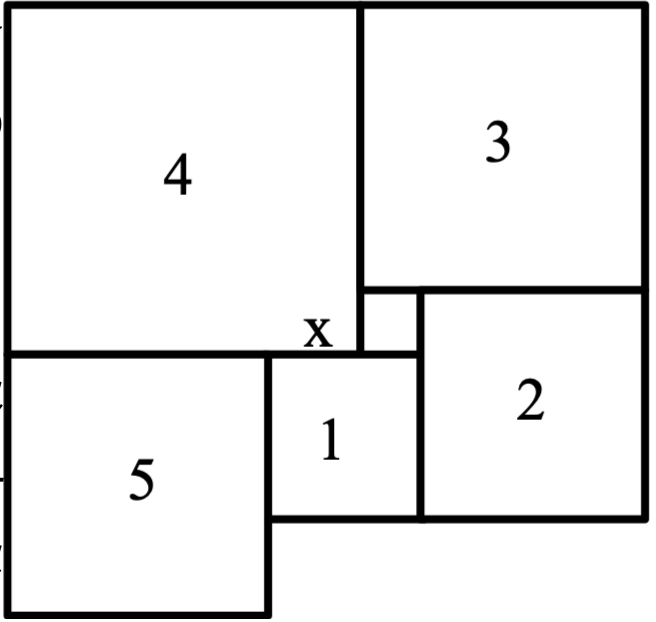
\includegraphics[width=\linewidth]{ЭлМШ 2025-2026/I блок/7/ВВП.png}
\end{wrapfigure}

\textbf{Решение:} Обозначим часть стороны квадрата $(1)$ $x$ так, чтобы сторона квадрата $(1)$ стала $(x+1)$, тогда сторона квадрата $(2)$ --- $(x+2)$ , сторона квадрата $(3)$ $-$ $(x+3)$  и, наконец, сторона квадрата $(4)$ - $(x+4)$. Сторона квадрата $(5)$ меньше стороны квадрата $(4)$ на $x$. Значит сторона квадрата $(5)$ есть $(x+4) - x=4$.

\textit{Замечание.} Чему равен $x$ из решения найти нельзя. Это не удивительно - на самом деле по данным в задаче условиям найти $x$ (а значит и длины сторон квадратов 1,2,3,4) нельзя.

\problem{4}
Бумага расчерчена на клеточки со стороной 1. Ваня вырезал из неё по клеточкам прямоугольник и нашёл его площадь и периметр. Таня отобрала у него ножницы и со словами "Смотри, фокус!" вырезала с краю прямоугольника по клеточкам квадратик, квадратик выкинула и объявила: "Теперь у оставшейся фигуры периметр такой же, какая была площадь прямоугольника, а площадь - как был периметр!" Ваня убедился, что Таня права.

а) Квадратик какого размера вырезала и выкинула Таня?

б) Приведите пример такого прямоугольника и такого квадрата.

в) Прямоугольник каких размеров вырезал Ваня?

\textbf{Ответ:} а) $2\times2$.; б) см. рис. к пункту в) решения; в) $3\times10$ или $4\times6$.


\begin{wrapfigure}{r}{0.25\linewidth}
    \vspace{-7mm}
    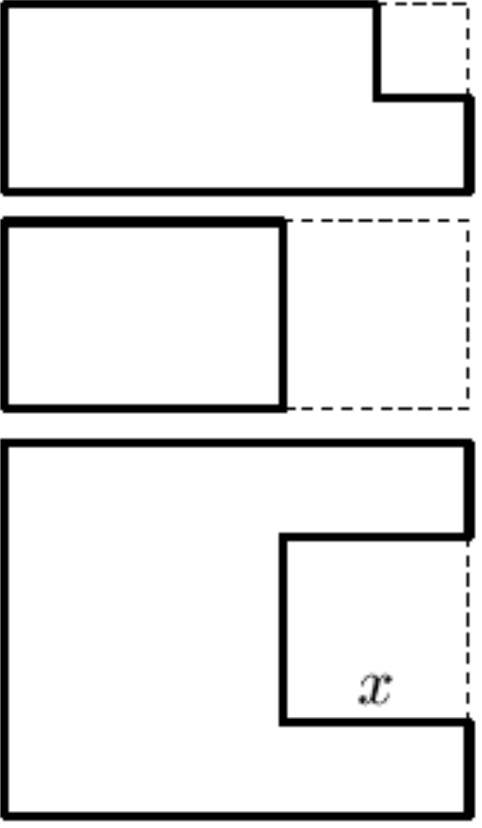
\includegraphics[width=\linewidth]{ЭлМШ 2025-2026/I блок/7/ВВП_2.png}
\end{wrapfigure}

\textbf{Решение.} а) Квадратик не мог иметь общий угол с прямоугольником (см. рис.), так как тогда периметр остался бы прежним или уменьшился (убедитесь сами!), а площадь бы уменьшилась. Значит квадрат примыкает только к одной из
сторон прямоугольника (см. рис.).

Пусть сторона квадрата $x$. Тогда Таня, вырезав квадрат, уменьшила площадь фигуры на $x^2$, при этом периметр увеличился на две стороны квадрата, то есть на $2x$. Таким образом, исходная площадь- $x^2=$ площадь полученной фигуры, исходный периметр $+2 x=$ периметр полученной фигуры. По условию исходная площадь = периметр полученной фигуры, исходный периметр $=$ площадь полученной фигуры.
Отсюда

исходная площадь --- $x^2=$ исходный периметр, 

исходный периметр $+\ 2 x=$ исходная площадь.

Значит, $x^2=2 x$, откуда $x=2$.

\newpage

\hspace{3mm}

\begin{wrapfigure}{r}{0.25\linewidth}
    \vspace{-7mm]}
    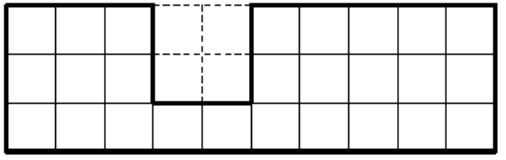
\includegraphics[width=\linewidth]{ЭлМШ 2025-2026/I блок/7/ВВП_4.png}
\end{wrapfigure}

в) Пусть стороны прямоугольника а и b. Тогда из решения пункта а) следует, что
площадь $=$ периметр +4 то есть, $a b=2 a+2 b+4$. Наша задача - найти все возможные пары чисел а и $b$, удовлетворяющие этому равенству. 

\begin{wrapfigure}{r}{0.25\linewidth}
    \vspace{-7mm]}
    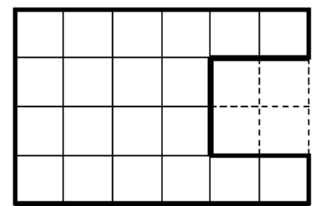
\includegraphics[width=\linewidth]{ЭлМШ 2025-2026/I блок/7/ВВП_3.png}
\end{wrapfigure}

Равенство $a b=2 a+2 b+4$ можно переписать как $(a-2)(b-2)=8$. Число 8 на множители разлагается двумя способами - $1 * 8$ и 2*4. Значит всего есть два варианта $a=3, b=10$ и $a=4, b=6$. Они указаны на рисунке.

\problem{5}
Турнир Солнечного города по шахматам проходил в один круг. В турнире принимали участие 100 коротышек. После турнира Незнайка неожиданно узнал, что за ничью давалось не $1 / 2$ очка, как он думал, а 0 очков, а за поражение - не 0 очков, а -1 , ну а за победу, как он считал и раньше, действительно начисляли 1 очко. В результате Незнайка набрал в два раза меньше очков, чем ему казалось. Сколько очков набрал Незнайка?

\textbf{Ответ:} 33 очка.

\textbf{Решение:} Раз турнир был круговым, то каждый сыграл с каждым, то есть Незнайка сыграл с 99 коротышками. Пусть Незнайка выиграл у а коротышек, сыграл в ничью с b коротышками и проиграл с коротышкам. Тогда $a+b+c=99$. Незнайка считал очки так:
$1 \cdot a+\frac{1}{2} \cdot b=\frac{2 a+b}{2}$, а нужно было считать так: $1 \cdot a+(-1) \cdot c=a-c$, что в 2 раза меньше по
подсчетам Незнайки. Таким образом верно следующее равенство: $\frac{2 a+b}{2}=2 a-2 c$. Преобразуем это равенство так: $a+b+c=3 a-3 c$. Известно, что $a+b+c=99$, Значит $a-c=33$, то есть Незнайка на шахматном турнире заработал 33 очка.